

\tikzset{every picture/.style={line width=0.75pt}} %set default line width to 0.75pt        

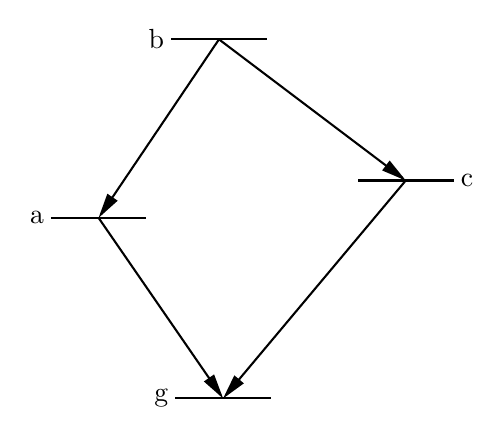
\begin{tikzpicture}[x=0.75pt,y=0.75pt,yscale=-1,xscale=1]
%uncomment if require: \path (0,300); %set diagram left start at 0, and has height of 300

%Straight Lines [id:da3132242130750498] 
\draw    (84,137) -- (130,137) ;
%Straight Lines [id:da8852176090904664] 
\draw    (232,119) -- (278,119) ;
%Straight Lines [id:da3118336041065983] 
\draw    (142,51) -- (188,51) ;
%Straight Lines [id:da13043475932345627] 
\draw    (144,224) -- (190,224) ;
%Straight Lines [id:da1403435354778697] 
\draw    (165,51) -- (108.12,135.34) ;
\draw [shift={(107,137)}, rotate = 304] [fill={rgb, 255:red, 0; green, 0; blue, 0 }  ][line width=0.08]  [draw opacity=0] (12,-3) -- (0,0) -- (12,3) -- cycle    ;
%Straight Lines [id:da048714045175360265] 
\draw    (165,51) -- (253.4,117.79) ;
\draw [shift={(255,119)}, rotate = 217.07] [fill={rgb, 255:red, 0; green, 0; blue, 0 }  ][line width=0.08]  [draw opacity=0] (12,-3) -- (0,0) -- (12,3) -- cycle    ;
%Straight Lines [id:da3087053085673217] 
\draw    (107,137) -- (165.86,222.35) ;
\draw [shift={(167,224)}, rotate = 235.41] [fill={rgb, 255:red, 0; green, 0; blue, 0 }  ][line width=0.08]  [draw opacity=0] (12,-3) -- (0,0) -- (12,3) -- cycle    ;
%Straight Lines [id:da2241090509364947] 
\draw    (255,119) -- (168.28,222.47) ;
\draw [shift={(167,224)}, rotate = 309.97] [fill={rgb, 255:red, 0; green, 0; blue, 0 }  ][line width=0.08]  [draw opacity=0] (12,-3) -- (0,0) -- (12,3) -- cycle    ;

% Text Node
\draw (280,119) node [anchor=west] [inner sep=0.75pt]   [align=left] {c};
% Text Node
\draw (82,137) node [anchor=east] [inner sep=0.75pt]   [align=left] {a};
% Text Node
\draw (142,224) node [anchor=east] [inner sep=0.75pt]   [align=left] {g};
% Text Node
\draw (140,51) node [anchor=east] [inner sep=0.75pt]   [align=left] {b};


\end{tikzpicture}
